% -*- coding: utf-8 -*-
 \documentclass[journal]{IEEEtran}
%\documentclass[titlepage, twocolumn, a4paper, 10pt]{article}
\usepackage[english]{babel}
\usepackage[utf8]{inputenc}
\usepackage{verbatim}
\usepackage{fancyhdr}
\usepackage{graphicx}
\usepackage{parskip}
\usepackage{url}

\usepackage[pdfborder={0 0 0 0}]{hyperref}

% Column spacing
\setlength{\columnsep}{7mm}

% Include pdf with multiple pages ex \includepdf[pages=-, nup=2x2]{filename.pdf}
\usepackage[final]{pdfpages}

% Place figures where they should be use [H]
\usepackage{float}

% Float for text
\floatstyle{ruled}
\newfloat{code}{H}{lop}
\floatname{code}{CodeSnippet}

% vars
\def\title{GCom}
\def\preTitle{Deliverable 2}
\def\kurs{Distributed systems, HT-09}


\def\namn{Anton Johansson}
\def\mail{dit06ajn@cs.umu.se}

\def\namnTva{Jonny Strömberg}
\def\mailTva{dit06jsg@cs.umu.se}


\def\pathtocode{\url{~/dit06ajn/edu/dist/GCom}}

\def\handledareEtt{Lars Larsson, larsson+ds@cs.umu.se}
\def\handledareTva{Daniel Henriksson, danielh+ds@cs.umu.se}

\def\inst{Computer Science}
\def\dokumentTyp{Report}

\begin{document}
\begin{titlepage}
  \thispagestyle{empty}
  \begin{small}
    \begin{tabular}{@{}p{\textwidth}@{}}
      UMEÅ UNIVERSITY \hfill \today \\
      Department of \inst \\
      \dokumentTyp \\
    \end{tabular}
  \end{small}
  \vspace{10mm}
  \begin{center}
    \LARGE{\preTitle} \\
    \huge{\textbf{\kurs}} \\
    \vspace{10mm}
    \LARGE{\title} \\
    \vspace{15mm}
    \begin{large}
      \namn, \mail \\
      \namnTva, \mailTva\\
      \texttt{\pathtocode}
    \end{large}
    \vfill
    \large{\textbf{Supervisors}}\\
    \mbox{\large{\handledareEtt}}\\
    \mbox{\large{\handledareTva}}
  \end{center}
\end{titlepage}

\newpage
\mbox{}
\vspace{70mm}
\begin{center}
  % Dedication goes here
\end{center}
\thispagestyle{empty}
\newpage

\pagestyle{fancy}
\rhead{\today}
\lhead{\footnotesize{\namn, \mail\\\namnTva, \mailTva}}
\chead{}
\lfoot{}
\cfoot{}
\rfoot{}

\cleardoublepage
\newpage
\onecolumn
\tableofcontents
\twocolumn
\cleardoublepage

\fancyfoot[LE,RO]{\thepage}
\pagenumbering{arabic}

\section{Introduction}\label{sec:intro}
% Beskriv med egna ord vad uppgiften gick ut på. Är det någonting som
% varit oklart och ni gjort egna tolkningar så beskriv dessa.
This report explains a solution for implementing a distributed
group communications middleware.

A distributed system is composed of separated processes that
coordinate activities by passing messages and a middleware is a
software layers that enables rapid development of other software by
supplying simple method-calls that hides the underlying implementation
details off the middleware.

The middleware described in this report is called \textit{GCom} and
provides an API\footnote{Application programming interface} for group
communication with different message sending/delivery rules. Two
communication methods are implemented: \textit{Reliable multicast},
\textit{Basic multicast}, described in greater detail in section
\ref{sec:communications-module}.

Four message-ordering types are implemented: \textit{Non-ordered},
\textit{First in first out}, \textit{Casual}, \textit{Total} and
\textit{Casual-Total}, described in greater detail in section
\ref{sec:message-ordering-module}.

The system is implemented in the programming language
\textit{Java}\footnote{\url{http://java.sun.com/}} and uses \textit{Java
  RMI}\footnote{\url{http://java.sun.com/javase/technologies/core/basic/rmi/index.jsp}}
for network communication.

The original specification of this practical assignment can be found at:\\
\begin{footnotesize}
  \url{http://www.cs.umu.se/kurser/5DV020/HT09/assignment.html}
  \footnote{Fetched \today} % DONE check
\end{footnotesize}

\section{Problem analysis}\label{sec:problem-analysis}
% As this project emphasizes analysis and investigation of a loosely
% specified problem, include any assumptions you made during the
% analysis phase in your report. Also discuss problems encountered and
% alternative solutions considered in the analysis. The report should
% also discuss to what extent the requirement list is fulfilled, as
% well as to which extent you could adhere to the the project plan.
The group communication for \textit{GCom} is specified to be a
distributed system, which means there can be no central server that
coordinates all activities for individual group members. Four guidance
on how to implement such a system the book \textit{Distributed
  Systems: Concepts and Design}\cite{book:dist-syst} list three
important consequences of a distributed system:

\begin{itemize}
\item \textbf{Concurrency: } Program execution are concurrent. In the
  case of \textit{GCom}, message receiving and handling are concurrent
  with other parts of the middleware such as message sending and ordering.
\item \textbf{No global clock: } There is no global clock to
  coordinate activities by. That is clock timestamps can not be used
  to order messages received by \textit{GCom}.
\item \textbf{Independent failures: } All individual parts of the
  distributed system can fail at any time and place in execution. This
  must be considered when implementing algorithms for coordinated
  actions of \textit{GCom}.
\end{itemize}

The environment in which \textit{GCom} will execute will defined by
a model for distributed system called \textit{asynchronous}-system
defined by three assumptions \cite{book:dist-syst}:

\begin{itemize}
\item There is no guarantee of \textbf{execution speed}, a process may respond
  to a request immediately or after several years.
\item In a similar manner there can be \textbf{transmission delays} in the
  network were messages are passed. A message can take arbitrary long
  time to arrive at its destination.
\item As stated before, there is \textbf{no global clock}. One process can make
  no assumptions about the clock in another process.
\end{itemize}

\subsection{Group partitioning}\label{sec:group-partitioning}
When considering the previous characteristics of the environment for
\textit{GCom}, a group of processes can at any time be divided in two
groups without any means for communication between them. It would be
impossible for the groups to determine whether the group members of
the other group still executes and behaves normally. Therefore a
partition of a group is treated as a crash of all the members cut off.
This means that merging such a group when communication can be
achieved again is done by a new join for all the members in one off
the groups.

% TODO: both groups will get new leaders, GNS should handle this and
% make the group without leader rejoin the previous group.

\subsection{Member failures}\label{sec:member-failures}
A member of a group is considered to have failed only when throws a
\textit{RemoteExceptioin}\footnote{\url{http://java.sun.com/javase/6/docs/api/java/rmi/RemoteException.html}}
as defined by \textit{Java RMI}. This means that \textit{GCom} makes
no guarantee about the time it takes to send a message to a group.
This guarantee could be achieved simply by changing the definition of
a member failure to include a time-limit for message delivery.

\section{Usage}\label{sec:usage}
% Förklara var programmet och källkoden ligger samt hur man kompilerar,
% startar och använder det. Förklara även översiktligt vad som händer
% när man använder de olika kommandona. Det räcker alltså inte att
% skriva "man skriver 'ant' för att kompilera", utan det måste även ingå
% en liten förklaring om vad som egentligen händer när man kör ant och
% varför det fungerar. Använd Internet eller litteratur för att själva
% ta reda på den information ni tycker känns relevant, dels för
% rapportens skull och dels för er egen. Kom ihåg att skriva tydliga
% (vetenskapliga) referenser!
All files needed to use this middleware are located at:\\
\texttt{\pathtocode}

This catalog contains the following sub directories:
\begin{itemize}
\item The directory \verb!src! contains the source code.
\item The directory \verb!src/main/resources/! contains configuration
  files for standard behaviour of the compiled system, see section
  \ref{sec:configuration}
\item The directory \verb!src! contains the source code.
\item The directory \verb!bin! will, after a successful compilation,
  contain all the compiled sources as well as configuration files used
  by this middleware.
\item The directory \verb!lib! contains all requires third-party libraries
  needed by \textit{GCom}, se section \ref{sec:required-libraries}.
\item The directory \verb!doc! contains the Javadoc API for \textit{GCom}.
\end{itemize}

\section{Compilation}\label{sec:compilation}
The following commands will require the software tool \textit{Apache
  Ant}\footnote{http://ant.apache.org/}. More details about what
happens using \textit{ant} in this project is found in the file
\textit{build.xml}\footnote{http://ant.apache.org/manual/using.html}.

To compile \textit{GCom} issue the following command:\\
\begin{footnotesize}
  \verb!salt:./GCom> ant!
\end{footnotesize}\\
This will create a directory \verb!bin! if it does not already exists
and compile/move source-code and configuration files to that
directory.

The root-directory for class-files when using \textit{GCom} is
compiled to \textit{bin/main/java}, while the root-directory for
test-code is compile to \textit{bin/test/java}.

To create \textit{jar}-file of the compiled sources issue the
following command:\\
\begin{footnotesize}
  \verb!salt:./GCom> ant jar!
\end{footnotesize}\\
This will create \textit{GCom.jar} which can be used when developing
in third party software or directly as a \textit{GNS}-server (see
section \ref{sec:group-naming-system}) by
running:\\
\begin{footnotesize}
  \verb!salt:./GCom> java -jar GCom.jar!
\end{footnotesize}

\subsection{Configuration}\label{sec:configuration}
The compiled system uses two configuration-files to define its
standard behaviour, these files are located in the directory
\textit{src/main/resources/}.

\subsubsection{application.properties}\label{sec:application.properties}
The file \textit{application.properties} defines the standard
multicast and ordering types to use when communication with a group.
Notice though that these settings are only used for the creator of a
group that did not exist from before. When connection to an existing
group, the settings from that group will suppress the settings in
\textit{application.properties}. CodeSnippet \ref{code:app-prop}
shows the content of an example configuration that uses

\begin{code}
  \begin{footnotesize}
\begin{verbatim}
# Used by GNS
gcom.gns.port=1078

# FIFO, TOTAL_ORDER, NO_ORDERING,
# CASUAL_ORDERING, CASUALTOTAL_ORDERING
gcom.ordering=FIFO

# BASIC_MULTICAST, RELIABLE_MULTICAST
gcom.multicast=RELIABLE_MULTICAST
\end{verbatim}
  \end{footnotesize}
  \caption{applications.properties}\label{code:app-prop}
\end{code}

\subsection{Required libraries}\label{sec:required-libraries}
Internally \textit{GCom} uses some third party software located in the
\textit{lib} directory and described in the following sections.

\subsection{SLF4J and Logback}\label{sec:logback}

\subsection{JUnit}\label{sec:junit}
For testing the individual parts of \textit{GCom}, tests are written
using the \textit{JUnit testing
  framework}\footnote{http://www.junit.org/}.

\section{System description}\label{sec:system}
% Beskriv översiktligt hur programmet är uppbyggt och hur det löser
% problemet.

% The GCom middleware consists of three (logical) modules, the group
% management module, the communication module and the message ordering
% module. These are, respectively, responsible for handling group
% membership issues, communication message exchange semantics and
% message (re)ordering issues. All of these modules need to function
% properly in order for your system to be able to ensure correct
% message delivery semantics.

% \begin{figure}[!t]
%   \centering
%   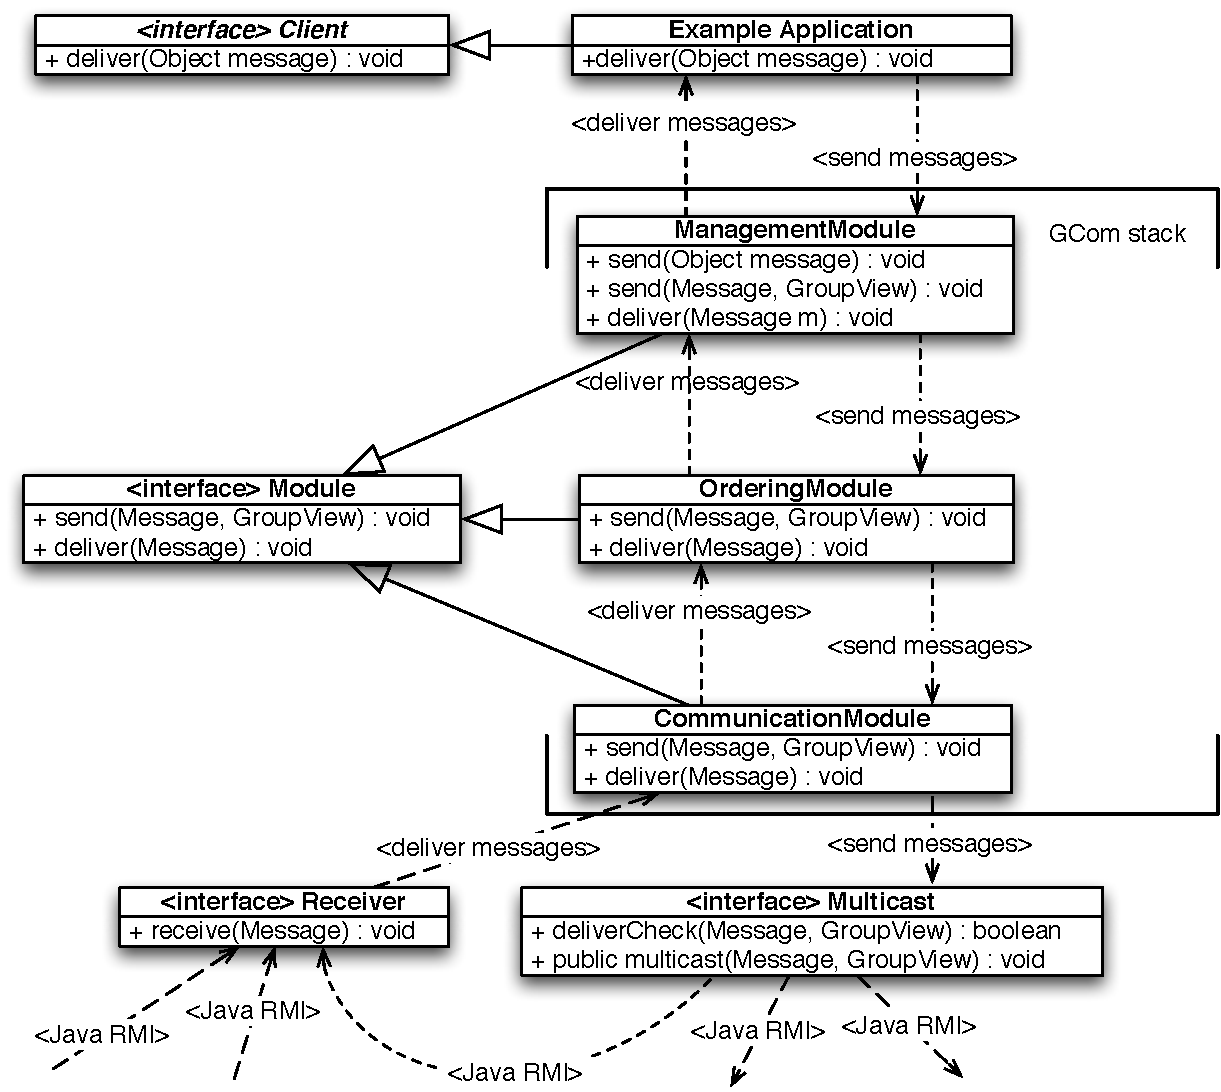
\includegraphics[width=2.5in]{images/Stack.pdf}
%    %   \centerline{\subfloat[Case I]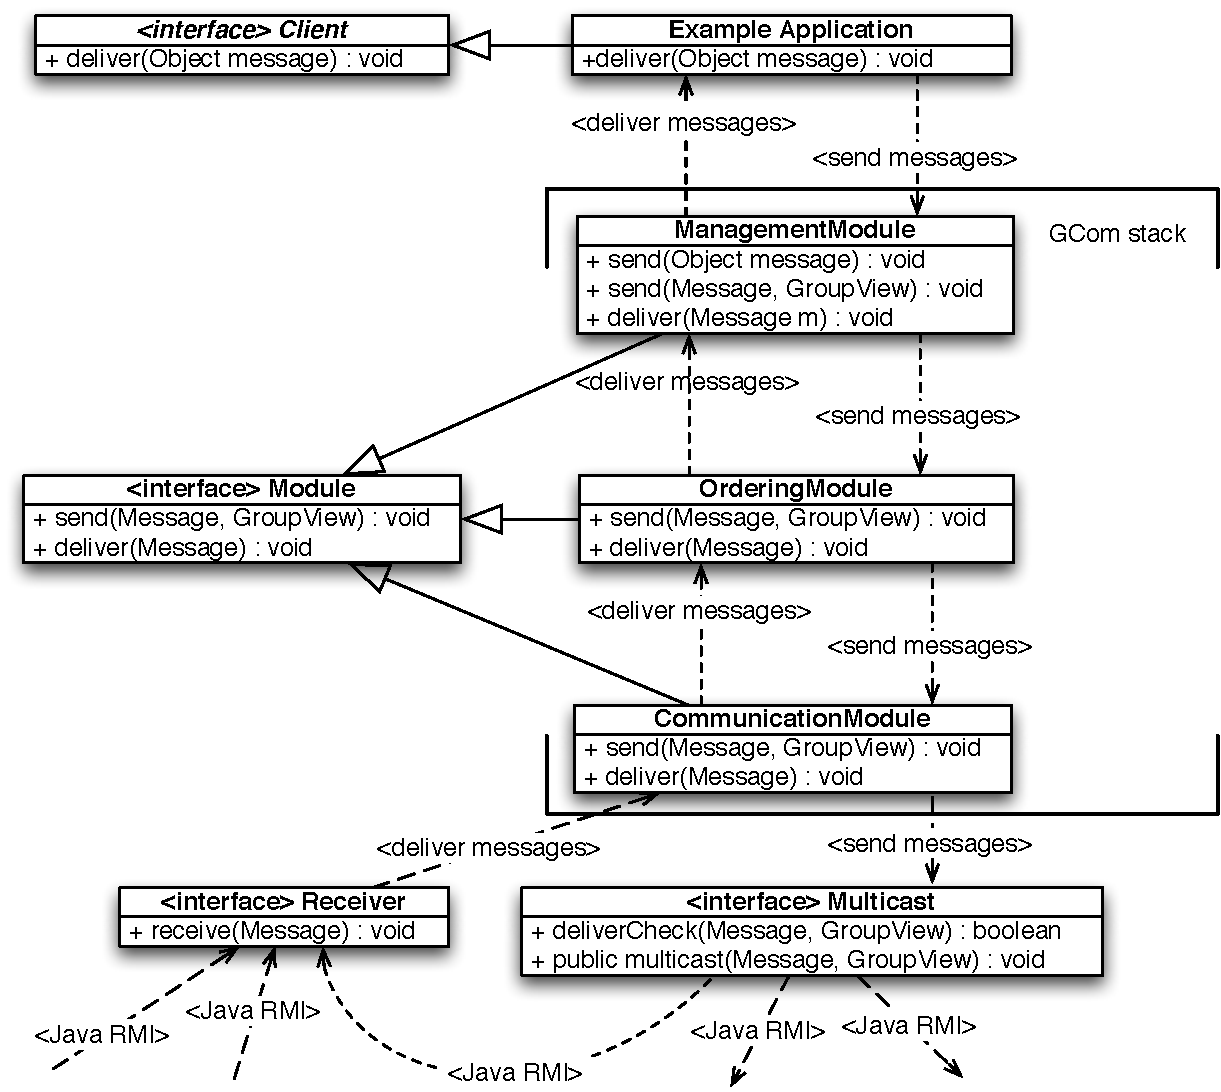
\includegraphics[width=2.5in]{images/Stack.pdf}}
%   \caption{GCom stack}
%   \label{fig:images/Stack}
% \end{figure}

\begin{figure*}[!t]
  \centerline{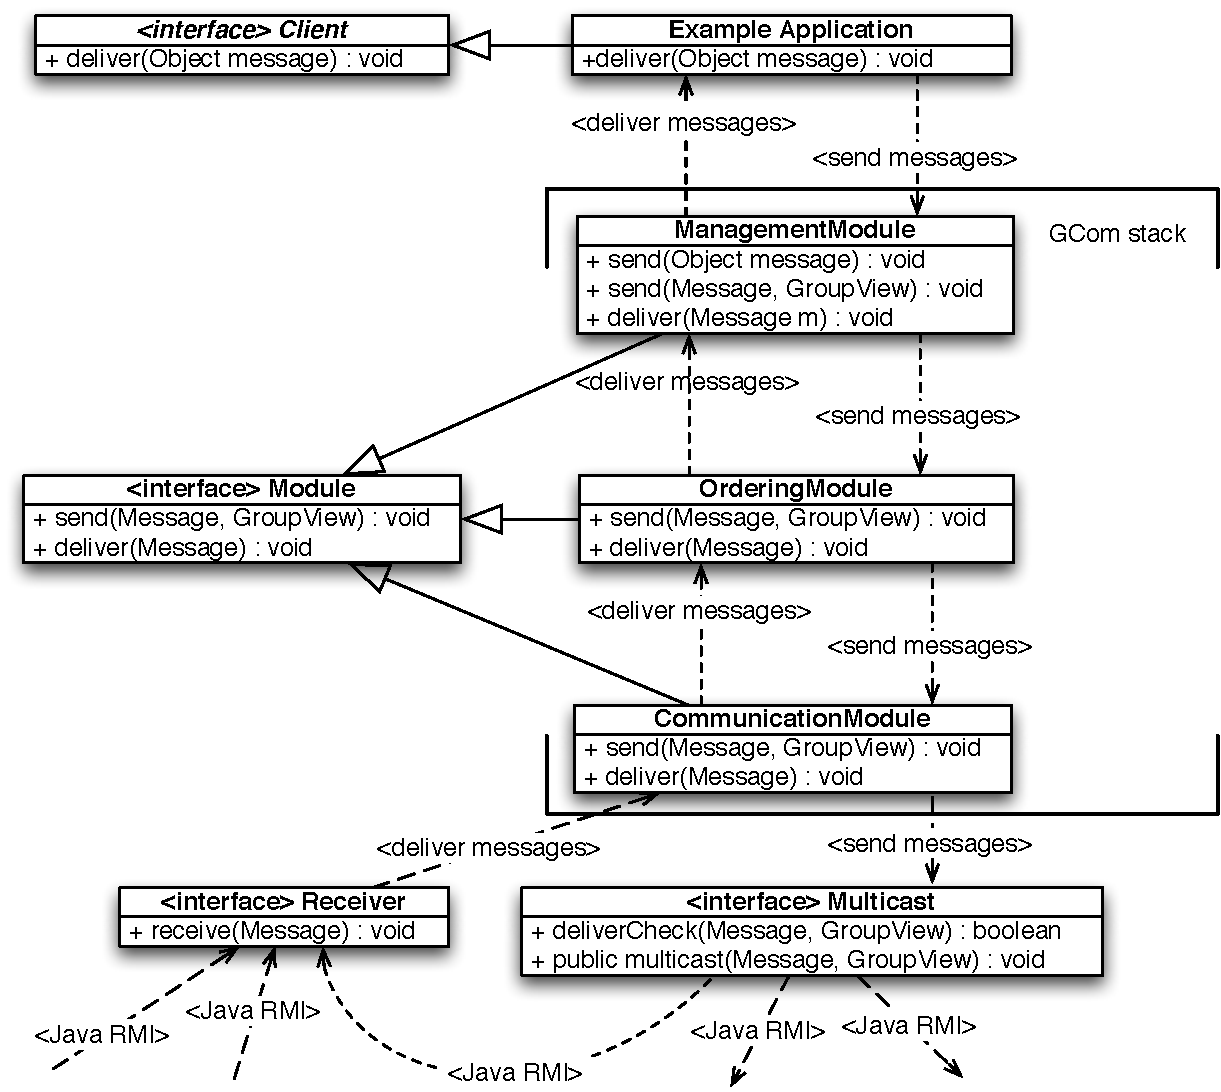
\includegraphics[width=110mm]{images/Stack.pdf}}
  \caption{GCom stack}
  \label{fig:images/Stack}
\end{figure*}



\subsection{Group management module}\label{sec:group-management-module}

\subsubsection{Group Naming System}\label{sec:group-naming-system}
% To resolve group names: When a process sends a message to the group,
% the group management module resolves the group name into a list of
% group members.

\subsubsection{Group leaders}\label{sec:group-leaders}
% To provide an interface for group management: The group management
% module provides operations to create and remove groups, as well as
% add and remove members from a group.

\subsubsection{Error handling}\label{sec:error-handling}
% To detect errors: The module monitors a group and indicates when a
% member of the group crashes (or for some other reason become
% unreachable).

\subsubsection{Group changes}\label{sec:group-changes}
% To notify changes in group membership: The module notifies all group
% members about changes in group composition.


\subsection{Communications module}\label{sec:communications-module}
\subsubsection{Basic multicast}\label{sec:basic-multicast}
\subsubsection{Reliable multicast}\label{sec:reliable-multicast}


\subsection{Message ordering module}\label{sec:message-ordering-module}
\subsubsection{Non-ordered}\label{sec:-non-ordered}
\subsubsection{FIFO}\label{sec:fifo}
\subsubsection{Causal}\label{sec:causal}
\subsubsection{Total}\label{sec:total}
\subsubsection{Causal-Total}\label{sec:causal-total}
% (messages are first sorted according to causal ordering, then according to total ordering)


\subsection{Debugger}\label{sec:debugger}
% That messages are delivered according to the specified ordering

% How messages are propagated in the network: Show both the path a
% message takes and how many times a certain process has received a
% certain message.

% The content of hold-back queues and other buffers: Present all
% messages waiting to be sent or delivered as well as values of vector
% clocks and other counters.

% Current system performance: As a measure of the system performance,
% count the number of messages (including control messages) required
% to perform an operation (send one message with certain ordering and
% certain multicast).


\section{Limitations}\label{sec:limitations}
% Vilka problem och begränsningar har din lösning av uppgiften? Hur
% skulle de kunna rättas till?

% \section{Reflektioner}\label{Reflektioner}
% % Reflektioner - Var det något som var speciellt krångligt? Vilka
% % problem uppstod och hur löste ni dem? Vilka verktyg använde ni? Hur
% % upplevde ni de verktygen? + Allmänna synpunkter. Om ni har upplevt
% % problem på grund av olika miljöer (i termer av operativsystem och
% % liknande) så kan det även vara intressant att nämna det, samt motivera
% % ert val av miljö.

\section{Tests}\label{sec:tests}
% Noggranna testkörningar där man ser att programmet fungerar som det
% ska.

% During your demo, you will need to convince the teachers that your
% implementation works. Bring a test protocol, i.e., a series of tests
% that clearly demonstrates that your GCom fulfills the requirements
% and a test tool which can be used to apply it. The test protocol
% should include, e.g., tests of all message orders and multicast
% types. Bring a copy of the test protocol on paper, see page 491 in
% [DS] for suggested notation. Your test protocol must clearly state
% your names, user names, and which level you intend to demonstrate.

% The fact that a system cannot be formally proven to work does not
% make it impossible to implement - consider for example the Internet.
% Read pages 498 and 508 in [DS].

%%%%%%%%%%%%%%%% END APPENDIX AND STUFF %%%%%%%%%%%%%%%%
\bibliographystyle{alpha}
\bibliography{books.bib}

\newpage
\appendix
\pagenumbering{roman}
\section{Appendix}\label{sec:kallkod}
% Källkoden ska finnas tillgänglig i er hemkatalog
% ~/edu/apjava/lab1/. Bifoga även utskriven källkod.

\end{document}
